\section{Condensatore piano: calcolare l'andamento del campo
	elettrico, e del potenziale dentro e fuori il condensatore e la
	sua capacità.}
Il condensatore piano \`e un sistema costituito da due superfici $piane$ di materiale conduttore, di superficie $S$, posti a una distanza $d$ e in modo da costituire due piani paralleli. Inoltre una superficie \`e caricata positivamente e l'altra negativamente.\\
\begin{center}
	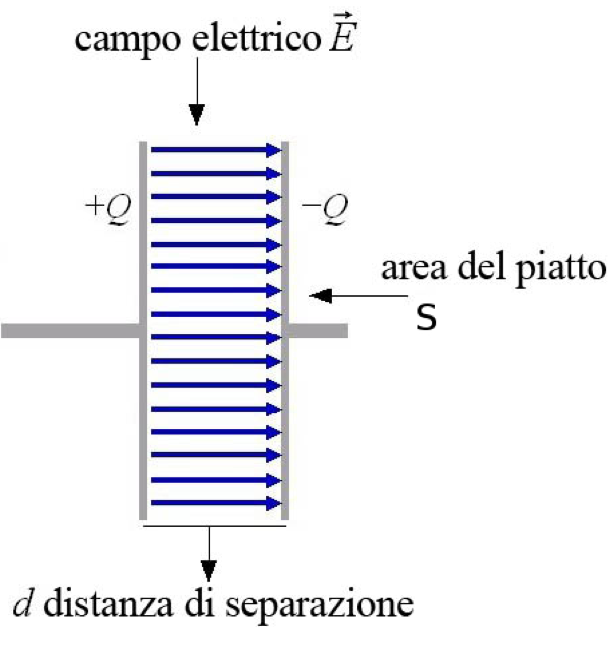
\includegraphics[height=5cm]{condensatore_piano}
\end{center}
\textbf{Esempio grafico :} come si puo' notare, all'interno di un condensatore piano vi \`e un campo elettrico uniforme.\\
Si definisce come \textbf{Capacit\'a} di un condensatore la quantit\'a di carica immagazzinabile sulle armature per unit\'a di differenza di potenziale ai capi delle armature.\\
$$
    C = \frac{Q}{\Delta V}
$$
All'esterno del condensatore il campo elettrico \`e nullo, poich\'e esso \`e isolato. $\left(\vec{E} = 0\right)$
Per calcolare il campo elettrico all'interno sfruttiamo il \textbf{Teorema di Gauss per il campo elettrico}: \\
\`E il caso della distribuzione piana di carica, assumiamo $\sigma$ come densita piana di carica:
$$
   \left[\sigma\right] = \left[\frac{Q}{L^2}\right]
$$
Intersechiamo un cilindro di raggio $r$ e lunghezza $l$ con un piano del condensatore, in modo tale che esso abbia entrambe le basi parallele al piano.

\pagebreak

Grazie a cio' possiamo affermare che il contributo al flusso delle basi \`e nullo, mentre \`e massimizzato sulla superficie laterale(dove le linee di campo sono perpendicolari).\\
$$
    \Phi(\vec{E}) = \frac{\sum{Q_{interne}}}{\varepsilon_0} = \oint_S{\vec{E} \cdot \hat{n}}
$$
Formalizziamo la affermazione precedente:
$$
    S = 2 S_{base} = \pi r^2
$$
inoltre si ha che
$$
    \sum{Q_{interne}} = \sigma S_{base}
$$
e calcoliamo il campo elettrico:
$$
    \frac{\sum{Q_{interne}}}{\varepsilon_0} = \oint_S{\vec{E} \cdot \hat{n}}
$$
$$
    \frac{\sigma S_{base}}{\varepsilon_0} = \oint_S{E}
$$
$$
    \frac{\sigma \cancel{S}}{\varepsilon_0} = 2 E \cancel{S}
$$
$$
    E = \frac{\sigma}{2 \varepsilon_0}
$$
Si noti che il capo elettrico in realt\'a \`e per una sola delle armature, pertanto 
$$
    E_{totale} = 2 E = \cancel{2} \frac{\sigma}{\cancel{2} \varepsilon_0} = \frac{\sigma}{\varepsilon_0}
$$
Per il calcolo della Capacit\'a bisogna calcolare la differenza di potenziale $\Delta V$ come :
$$
    \Delta V = \int_{A}^{B}{\vec{E} \cdot \vec{ds}} = \frac{\sigma}{\varepsilon_0}d
$$
Dove $d$ \`e la distanza fra le armature.\\
Pertanto:
$$
    C = \frac{Q}{\Delta V} = Q \frac{\varepsilon_0}{\sigma d} = 
    \cancel{\sigma} S \frac{\varepsilon_0}{\cancel{\sigma} d} = \frac{S\varepsilon_0}{d}
$$
$\hfill\square$